\documentclass[journal,12pt,twocolumn]{IEEEtran}

\usepackage{setspace}
\usepackage{gensymb}
\singlespacing
\usepackage[cmex10]{amsmath}

\usepackage{amsthm}
\usepackage{karnaugh-map}
\usepackage{mathrsfs}
\usepackage{txfonts}
\usepackage{stfloats}
\usepackage{bm}
\usepackage{cite}
\usepackage{cases}
\usepackage{subfig}
\usepackage{float}
\usepackage{longtable}
\usepackage{multirow}

\usepackage{enumitem}
\usepackage{mathtools}
\usepackage{steinmetz}
\usepackage{tikz}
\usepackage{circuitikz}
\usepackage{verbatim}
\usepackage{tfrupee}
\usepackage[breaklinks=true]{hyperref}
\usepackage{graphicx}
\usepackage{tkz-euclide}

\usetikzlibrary{calc,math}
\usepackage{listings}
    \usepackage{color}                                            %%
    \usepackage{array}                                            %%
    \usepackage{longtable}                                        %%
    \usepackage{calc}                                             %%
    \usepackage{multirow}                                         %%
    \usepackage{hhline}                                           %%
    \usepackage{ifthen}                                           %%
    \usepackage{lscape}     
\usepackage{multicol}
\usepackage{chngcntr}

\DeclareMathOperator*{\Res}{Res}

\renewcommand\thesection{\arabic{section}}
\renewcommand\thesubsection{\thesection.\arabic{subsection}}
\renewcommand\thesubsubsection{\thesubsection.\arabic{subsubsection}}

\renewcommand\thesectiondis{\arabic{section}}
\renewcommand\thesubsectiondis{\thesectiondis.\arabic{subsection}}
\renewcommand\thesubsubsectiondis{\thesubsectiondis.\arabic{subsubsection}}


\hyphenation{op-tical net-works semi-conduc-tor}
\def\inputGnumericTable{}                                 %%

\lstset{
%language=C,
frame=single, 
breaklines=true,
columns=fullflexible
}
\begin{document}


\newtheorem{theorem}{Theorem}[section]
\newtheorem{problem}{Problem}
\newtheorem{proposition}{Proposition}[section]
\newtheorem{lemma}{Lemma}[section]
\newtheorem{corollary}[theorem]{Corollary}
\newtheorem{example}{Example}[section]
\newtheorem{definition}[problem]{Definition}

\newcommand{\BEQA}{\begin{eqnarray}}
\newcommand{\EEQA}{\end{eqnarray}}
\newcommand{\define}{\stackrel{\triangle}{=}}
\bibliographystyle{IEEEtran}
\raggedbottom
\providecommand{\mbf}{\mathbf}
\providecommand{\pr}[1]{\ensuremath{\Pr\left(#1\right)}}
\providecommand{\qfunc}[1]{\ensuremath{Q\left(#1\right)}}
\providecommand{\sbrak}[1]{\ensuremath{{}\left[#1\right]}}
\providecommand{\lsbrak}[1]{\ensuremath{{}\left[#1\right.}}
\providecommand{\rsbrak}[1]{\ensuremath{{}\left.#1\right]}}
\providecommand{\brak}[1]{\ensuremath{\left(#1\right)}}
\providecommand{\lbrak}[1]{\ensuremath{\left(#1\right.}}
\providecommand{\rbrak}[1]{\ensuremath{\left.#1\right)}}
\providecommand{\cbrak}[1]{\ensuremath{\left\{#1\right\}}}
\providecommand{\lcbrak}[1]{\ensuremath{\left\{#1\right.}}
\providecommand{\rcbrak}[1]{\ensuremath{\left.#1\right\}}}
\theoremstyle{remark}
\newtheorem{rem}{Remark}
\newcommand{\sgn}{\mathop{\mathrm{sgn}}}
\providecommand{\abs}[1]{\left\vert#1\right\vert}
\providecommand{\res}[1]{\Res\displaylimits_{#1}} 
\providecommand{\norm}[1]{\left\lVert#1\right\rVert}
%\providecommand{\norm}[1]{\lVert#1\rVert}
\providecommand{\mtx}[1]{\mathbf{#1}}
\providecommand{\mean}[1]{E\left[ #1 \right]}
\providecommand{\fourier}{\overset{\mathcal{F}}{ \rightleftharpoons}}
%\providecommand{\hilbert}{\overset{\mathcal{H}}{ \rightleftharpoons}}
\providecommand{\system}{\overset{\mathcal{H}}{ \longleftrightarrow}}
	%\newcommand{\solution}[2]{\textbf{Solution:}{#1}}
\newcommand{\solution}{\noindent \textbf{Solution: }}
\newcommand{\cosec}{\,\text{cosec}\,}
\providecommand{\dec}[2]{\ensuremath{\overset{#1}{\underset{#2}{\gtrless}}}}
\newcommand{\myvec}[1]{\ensuremath{\begin{pmatrix}#1\end{pmatrix}}}
\newcommand{\mydet}[1]{\ensuremath{\begin{vmatrix}#1\end{vmatrix}}}
\numberwithin{equation}{subsection}
\makeatletter
\@addtoreset{figure}{problem}
\makeatother
\let\StandardTheFigure\thefigure
\let\vec\mathbf
\renewcommand{\thefigure}{\theproblem}
\def\putbox#1#2#3{\makebox[0in][l]{\makebox[#1][l]{}\raisebox{\baselineskip}[0in][0in]{\raisebox{#2}[0in][0in]{#3}}}}
     \def\rightbox#1{\makebox[0in][r]{#1}}
     \def\centbox#1{\makebox[0in]{#1}}
     \def\topbox#1{\raisebox{-\baselineskip}[0in][0in]{#1}}
     \def\midbox#1{\raisebox{-0.5\baselineskip}[0in][0in]{#1}}
\vspace{3cm}
\title{FPGA Lab Project}
\author{Sachinkumar Dubey - EE20MTECH11009}
\maketitle
\newpage
\bigskip
\renewcommand{\thefigure}{\theenumi}
\renewcommand{\thetable}{\theenumi}
\noindent Download all codes from 
\begin{lstlisting}
https://github.com/sachinomdubey/FPGA_Lab/project_sachin/
\end{lstlisting}

\section{Step for Flashing ESP32}
\begin{itemize}
    \item Download the ESP32 webserver code from below link:\\
    \url{https://github.com/sachinomdubey/FPGA_Lab/tree/main/project_sachin/webserverESP32}
    \item ESP32 should connect to your android hotspot to host the webserver, for this make changes in below lines as per your hotspot credentials:
    \begin{lstlisting}
    const char* ssid = "SOD";
    const char* password = "sachin009";
    \end{lstlisting}
    \item We need to know the IP address of ESP32 to access the http web server. To know the IP address, also uncomment the below line in ESP32webserver code before flashing.
    \begin{lstlisting}
    //    Serial.println(WiFi.localIP());
    \end{lstlisting}
    \item Select the following settings in Arduino IDE before flashing:
    \begin{itemize}
        \item Board : ESP32 Dev Module
        \item Upload speed : 115200
        \item CPU frequency : 240 MHz
        \item Flash frequency : 40 MHz
        \item Flash size : 4 MB
    \end{itemize}
    \item Use TTL to USB connector to flash the code to ESP32. While flashing, connect IO0 pin of onboard ESP32 of Vaman to GND. Now press Upload on arduino IDE. While it says "connecting", connect the EN pin of ESP32 to GND for 1-2 Sec and subsequently disconnect the EN pin. The flashing process should start and complete.
    \item  After you reset, open the serial terminal where you can see the IP address. Note this down. 
    \item Repeat the flashing process by again commenting the below line. This is to make sure, it does not interfere when esp32 sends data to ARM UART.
    \begin{lstlisting}
    //    Serial.println(WiFi.localIP());
    \end{lstlisting}
\end{itemize}
\section{Step for Flashing Vaman ARM}
\begin{itemize}
    \item Download the Vaman code from below link:\\
    \url{https://github.com/sachinomdubey/FPGA_Lab/tree/main/project_sachin/Vaman_Signal_Processing}
    \item On terminal, Run "make" command in GCC\_project folder to generate .bin file.
    \item Flash the .bin file along with top.bin to vaman using following command. NOTE: change directory paths and port as per your system.
    \begin{lstlisting}
    python3 /home/sachin/Documents/Vaman/qorc-sdk/TinyFPGA-Programmer-Application/tinyfpga-programmer-gui.py --port /dev/ttyACM0 --m4app /home/sachin/Documents/Vaman/project_sachin/GCC_Project/output/project_sachin.bin --appfpga /home/sachin/Documents/Vaman/top.bin --mode fpga-m4 --reset
    \end{lstlisting}
\end{itemize}
\section{Wiring Diagram}
\url{https://github.com/sachinomdubey/FPGA_Lab/blob/main/project_sachin/Figures/FPGA_lab_project_wiring.pdf}
\section{Checking the result}
\begin{itemize}
    \item Make connections as per the wiring diagram.
    \item Reset the controller.
    \item ESP32 gets connected to Android hotspot automatically.
    \item Go the IP address which was acquired during flashing project in chrome browser. you can observe the following interface.
    \begin{figure}[ht]
    \centering
    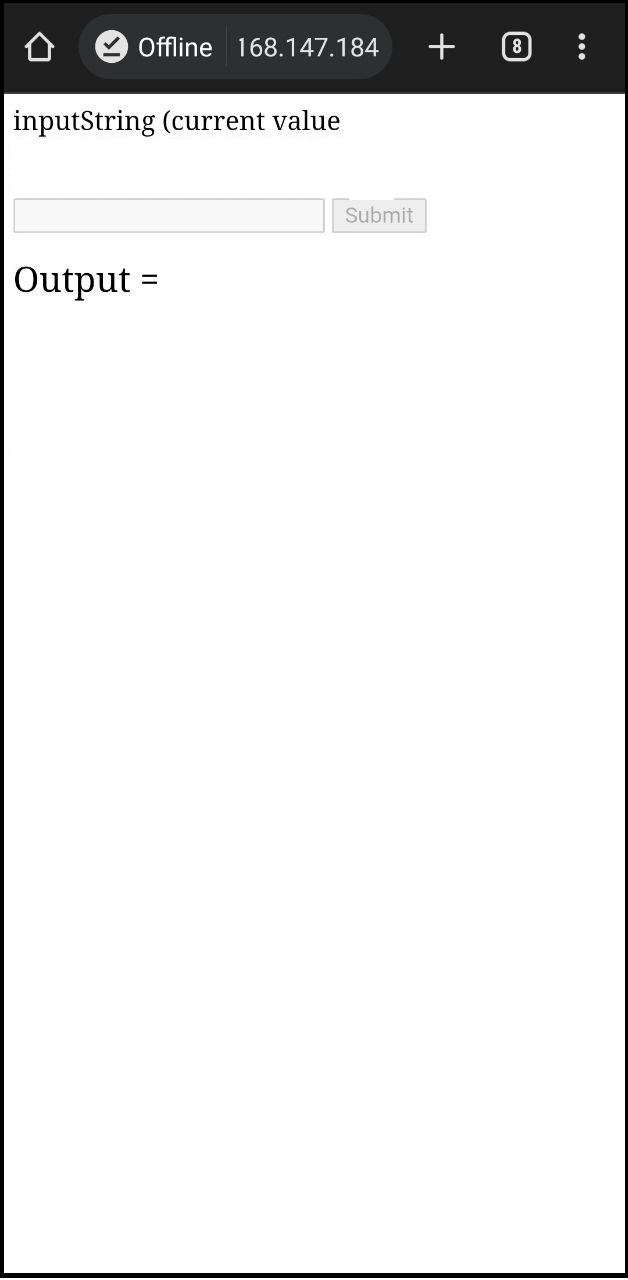
\includegraphics[width = 6.5cm]{Figures/Fig1.png}
    \end{figure}
    \newpage
    \item Enter the signal samples x[n] you want to convolve or correlate and press submit. (Note: we are sending the x[n] and h[n] is defined inside the ARM code itself). A sample x[n] and the expected output y[n] is given below.
    \begin{lstlisting}
x[n] = 0.5377, 1.8339, -2.2588, 0.8622, 0.3188, -1.3077, -0.4336, 0.3426, 3.5784, 2.7694, -1.3499, 3.0349, 0.7254, -0.0631, 0.7147, -0.2050, -0.1241, 1.4897, 1.4090, 1.4172
    \end{lstlisting}
    \begin{lstlisting}
convolution y[n] = 0.3611 0.5822 -3.3456 5.4983 0.8055 -2.8740 4.1062 -0.4103 -1.4459 -1.8042 -4.3505 13.2034 -2.7157 4.8211 10.2696 -4.4270 9.7560 2.9032 -0.5928 4.6351 -7.3842 0.3368 -9.3994 -8.5450 3.6132 -9.3192 -3.9125 0.5994 -3.3785 -1.2455 -3.9723 -7.0416 -5.2957 -4.1727  
    \end{lstlisting}
    \begin{lstlisting}
correlation y[n] = -1.5832  -5.8348  4.5913  -3.2871  -0.8481  6.4676  -2.2871  3.2946  -10.0747  -9.5041  -1.4903  -14.6805  0.2470  -5.4371  -12.3220  7.0057  -4.8595  0.2204  0.6648  0.1413  5.3020  -4.1038  2.3260  8.0337  -5.2602  3.1251  2.8166  1.9617  5.2222  4.0704  1.4387  0.3154  -0.7651  0.9516
    \end{lstlisting}
    \item The entered samples goes through ESP32 UART to ARM UART. ARM then performs the required operation (convolution or correlation) depending on the status of GPIO4 pin. 
    (GND - Convolution, 3.3V - Correlation)
    \item ARM sends the output back through ARM UART to ESP32 UART. ESP32 then display the output on webserver as shown in below figure:
    \begin{figure}[ht]
    \centering
    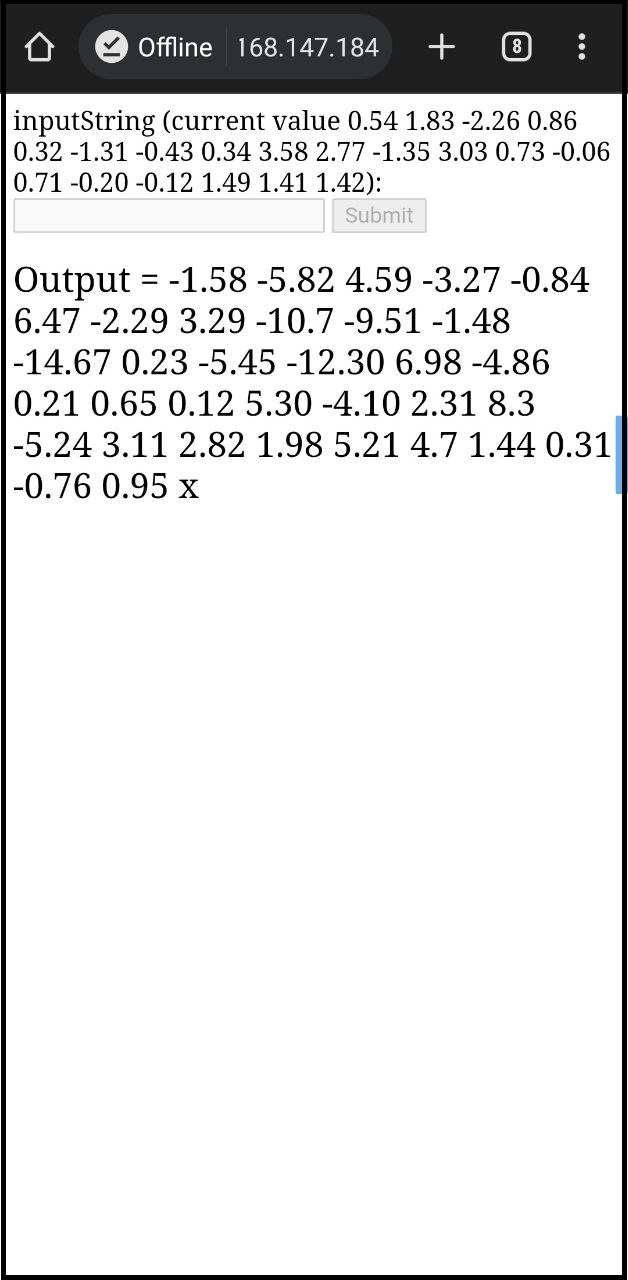
\includegraphics[width = 6.5cm]{Figures/Fig2.jpg}
    \end{figure}
\end{itemize}
\end{document}